% 2011 年湖南卷理科第 11 题：半圆三等分点与 AD⊥BC。
% 来源 PDF：普通高考/2011/2011湖南理.pdf，SHA-256 09b67f1db8e6a280165cf8431211a968163c0d0f262a50068dd607607a9ec578。
% 原页：第 1 页第 2 栏中部，书页码 671。
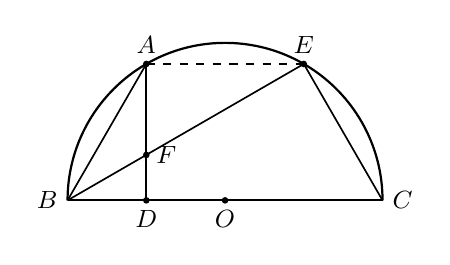
\begin{tikzpicture}[>=stealth, semithick, font=\small, scale=1.0]
  \draw[thick] (-2,0) arc (180:0:2);
  \draw[thick] (-2,0)--(2,0);
  \coordinate (B) at (-2,0); \coordinate (C) at (2,0);
  \coordinate (A) at (-1,1.732); \coordinate (E) at (1,1.732);
  \coordinate (D) at (-1,0); \coordinate (O) at (0,0);
  \coordinate (F) at (-1,0.577);
  \draw (A)--(D); \draw (A)--(B);
  \draw (B)--(E); \draw (E)--(C);
  \draw[dashed] (A)--(E);
  \fill (A) circle (1.2pt) node[above] {$A$};
  \fill (E) circle (1.2pt) node[above] {$E$};
  \fill (F) circle (1.2pt) node[right] {$F$};
  \fill (D) circle (1.2pt) node[below] {$D$};
  \fill (O) circle (1.2pt) node[below] {$O$};
  \node[left] at (B) {$B$};
  \node[right] at (C) {$C$};
\end{tikzpicture}
